% AQSE manuscript: Passes 1--5 working source for IEEE Transactions on Quantum Engineering.
% IEEEtran journal layout is used for this review draft. See README.md for template status.
\documentclass[journal]{IEEEtran}
\usepackage[T1]{fontenc}
\usepackage[utf8]{inputenc}
\usepackage{amsmath,amssymb}
\usepackage{cite}
\usepackage{graphicx}
\usepackage{booktabs}
\usepackage{tikz}
\usepackage[hidelinks]{hyperref}
\urlstyle{same}

\title{AQSE: A Hybrid Quantum--Classical Framework for Contextual Sensor-Network Representation}
% The author list, affiliations, funding, and ORCIDs require author confirmation.
% Do not infer them from repository ownership.
\author{}

\begin{document}
\maketitle
\begin{center}
\small\textit{Working draft. Core text complete through Conclusions; final integration pending.}
\end{center}
% Abstract, Index Terms, authors and final submission checks belong to final integration.
% The completed core text is not yet a submission-ready manuscript.

\section{Introduction}
\label{sec:introduction}

Magnetometer records combine the field of interest with environmental interference, instrument response, and measurement noise. A change in one record can therefore admit several explanations. Measurements from neighboring nodes can provide context, but redundancy alone does not make every environmental and instrumental cause identifiable. Multisensor fusion provides methods for combining such information~\cite{hall1997fusion}. Quantum sensing concerns a different layer: the use of quantum systems to measure physical quantities~\cite{degen2017sensing}. Here, the quantum computation acts on classical measurement features after readout. It does not alter the sensing interaction or establish an improvement in hardware sensitivity.

Quantum kernel methods provide one route for processing these features. A parameterized circuit maps an input vector to a quantum state, and state overlaps define a similarity function for a classical kernel predictor~\cite{schuld2019feature,havlicek2019supervised}. Training the circuit changes that similarity function. This creates two separate questions: whether optimization changes the representation, and whether the resulting representation improves prediction on unseen observations. A large state space answers neither question. The predictive value of a quantum kernel depends on the data and target, as well as on the available classical alternatives~\cite{huang2021power}. Benchmarking studies have reported task-dependent outcomes rather than a general benefit from quantum kernel training~\cite{alvarez2025benchmarking,schnabel2025scrutiny}.

AQSE is a hybrid quantum--classical framework for studying these questions in sensor-data processing. Its network demonstrator connects simulated observations from one to eight magnetometers to causal, eight-dimensional local or network feature profiles. An eight-qubit variational quantum circuit (VQC), with 16 trainable parameters, defines a trainable quantum kernel (TQK). The demonstrator converts kernel similarities to a fixed-dimensional classical representation using a regularized Nystr\"om map, termed AFSE within AQSE, and passes that representation to a multilayer perceptron (MLP). AFSE is an application of a classical kernel approximation, not a separate quantum algorithm~\cite{williams2001nystrom}. Training and inference are distinct operations. Quantum natural gradient (QNG) updates the circuit parameters during an explicit training job~\cite{stokes2020qng}; inference uses frozen parameters and preprocessing. Versioned model bundles link each output to its feature profile, scaler, circuit parameters, landmarks, and classifier~\cite{aqse2026canonical}.

The framework and the statistical benchmark have different scopes. The replicated experiment reported here isolates the TQK component on a controlled, single-magnetometer task: discrimination between nominal and elevated white-noise regimes under harmonic excitation. It uses an eight-feature harmonic representation and a support vector classifier (SVC) operating directly on the quantum kernel. It does not evaluate the complete network State8--AFSE--MLP path. The network architecture establishes the application context; the replicated benchmark tests a bounded component-level hypothesis. All quantum computations use exact statevector simulation. No quantum processing unit (QPU) or physical sensor deployment is evaluated.

The primary question is whether validation-selected TQK models outperform a radial basis function SVC (RBF-SVC) on held-out balanced accuracy within this simulated task. The protocol was versioned in the repository before execution. It specifies 30 independently generated primary replicas, each with 72 training, 24 validation, and 24 test episodes. Each episode contributes one fixed analysis window. Circuit optimization uses a balanced subset of 32 training examples; the final kernel SVC uses all 72 training examples. Preprocessing is fitted on training data, and checkpoint and hyperparameter selection uses validation data. Test evaluation follows the selection freeze. The comparator set includes RBF-SVC, a compact MLP, random Fourier features (RFF) with a linear SVC, and gradient boosting. Two additional control sets contain 12 runs each~\cite{aqse2026canonical}.

This paper makes three contributions. First, it describes a versioned sensor-processing framework that separates observable measurements, simulator-only causes, learned representations, and predictions. Second, it reports a repository-preregistered comparison of TQK learning and classical alternatives under a common episode-level data split. Third, it examines kernel spectra across optimization checkpoints and reports the controls alongside predictive results. These diagnostics describe representation and selection behavior; they are not substitutes for held-out evaluation.

The mean test balanced accuracy was 0.9528 for TQK and 0.9569 for RBF-SVC. Their paired difference was $-0.0042$, with a 95\% bootstrap interval of $[-0.0222,\,0.0125]$ and a two-sided Wilcoxon $p=0.933$. The preregistered predictive-advantage criterion was not met~\cite{aqse2026canonical}. The training-label permutation control also requires qualification: validation labels remained available for model selection. It is therefore a partial training-signal ablation, not a complete removal of supervised information. We interpret the results within these boundaries and distinguish changes in kernel geometry from evidence of predictive or computational advantage.

\section{Related Work}
\label{sec:related_work}

\subsection{Quantum Kernels and Task-Dependent Inductive Bias}

Schuld and Killoran~\cite{schuld2019feature} formulated quantum data encodings as feature maps, linking state preparation and overlap evaluation to classical kernel learning. Havl\'{i}\v{c}ek \emph{et al.}~\cite{havlicek2019supervised} implemented quantum feature-space learning on superconducting hardware. These studies established a mechanism for constructing kernels from quantum states. They did not establish that an arbitrary quantum feature map improves classification of arbitrary classical data.

For a pure-state encoding $|\psi_{\boldsymbol{\theta}}(\mathbf{x})\rangle$, the fidelity kernel used in AQSE is
\begin{equation}
 k_{\boldsymbol{\theta}}(\mathbf{x},\mathbf{x}') =
 \bigl|\langle\psi_{\boldsymbol{\theta}}(\mathbf{x})
 \mid\psi_{\boldsymbol{\theta}}(\mathbf{x}')\rangle\bigr|^2.
 \label{eq:fidelity-kernel}
\end{equation}
The circuit and encoding determine which inputs are similar under this kernel. Huang \emph{et al.}~\cite{huang2021power} showed why access to data changes quantum--classical learning comparisons: classical predictors can exploit samples even when reproducing an underlying quantum computation is difficult. Conversely, Liu \emph{et al.}~\cite{liu2021rigorous} established a supervised-learning separation for a constructed task under a classical hardness assumption. That result does not transfer without its assumptions to sensor-noise classification.

Problem structure can guide kernel construction. Glick \emph{et al.}~\cite{glick2024covariant} developed covariant kernels for data with group structure. Shin \emph{et al.}~\cite{shin2026tensor} characterized embedding quantum kernels through entangled tensor kernels, separating the roles of local data maps and a circuit-dependent core tensor. These perspectives connect inductive bias to the encoding and circuit structure. AQSE does not derive its circuit from a symmetry of the sensor task or establish classical intractability. Its claim is limited to evaluating a specified representation against declared comparators.

\subsection{Trainable Embeddings and Geometric Optimization}

The encoding itself constrains a variational model. Schuld \emph{et al.}~\cite{schuld2021encoding} related data-encoding gates to the accessible Fourier structure of the model. Repeated encoding can enlarge that structure, but additional expressivity does not determine generalization. Hubregtsen \emph{et al.}~\cite{hubregtsen2022training} optimized quantum embedding kernels through kernel-target alignment and studied finite-sampling and device-noise effects. Alignment supplies a training objective for the representation. It does not directly measure prediction error on a held-out population.

QNG uses the real part of the quantum geometric tensor to account for the local geometry of parameterized states~\cite{stokes2020qng}. AQSE uses a damped empirical Fubini--Study metric in its optimizer. This parameter-space metric must be distinguished from the spectrum of the Gram matrix over training examples. The former determines an update direction; the latter describes similarities between encoded samples. A change in either quantity is not, by itself, evidence of improved test performance.

Rodriguez-Grasa \emph{et al.}~\cite{rodriguez2025neural} proposed neural quantum kernels obtained from trained quantum neural networks. Their method learns an embedding before constructing the kernel matrix. AQSE instead optimizes a fidelity kernel through its declared alignment objective. Its downstream classical perceptron and Nystr\"om map belong to a separate integration path. In AQSE, the classical downstream model does not train the quantum embedding jointly with the kernel objective.

\subsection{Trainability, Bandwidth, and Kernel Concentration}

McClean \emph{et al.}~\cite{mcclean2018barren} identified regimes in which gradients of parameterized quantum circuits become exponentially small. Thanasilp \emph{et al.}~\cite{thanasilp2024concentration} analyzed exponential concentration of quantum kernel values under conditions involving the encoding, measurements, entanglement, or noise. These results concern scaling and estimation requirements under specified assumptions. They do not imply that every eight-qubit classifier suffers from the same failure mode.

Input scaling is another design variable. Shaydulin and Wild~\cite{shaydulin2022bandwidth} showed that quantum kernel bandwidth can affect generalization. In AQSE, preprocessing and its fitting population are therefore part of the model definition rather than incidental data preparation. The harmonic benchmark also treats phase as a circular coordinate, while the demonstrator's State8 profile has different semantics.

We use effective rank, the largest-eigenvalue fraction of the trace, and checkpoint-dependent spectra as finite-sample diagnostics. These quantities can expose simple empirical degeneracies. They do not measure task alignment on their own, quantify entanglement, or rule out concentration as qubit count increases. Exact-state simulation also excludes the shot-estimation and hardware-noise costs addressed in concentration and trainability analyses.

\subsection{Comparative Evaluation and Selection Effects}

In a direct TQE precedent, Alvarez-Estevez~\cite{alvarez2025benchmarking} compared quantum kernel estimation and training with different feature maps for classification. The study reported mixed task-dependent effects of training. Schnabel and Roth~\cite{schnabel2025scrutiny} examined fidelity and projected kernels across classification and regression problems. Their analysis identified roles for regularization, bandwidth, and other design choices. The preprint by Bowles \emph{et al.}~\cite{bowles2024benchmarking} compared several quantum model families with classical alternatives and emphasized the dependence of conclusions on datasets and benchmarking choices.

Prior work already covers broad model comparisons and spectral diagnostics. AQSE contributes a sensor-derived test case with a fixed replication count, recorded seeds, episode-level partitions, and an explicit selection-before-test sequence. Its comparator set spans kernel, neural, random-feature, and ensemble models. The comparison does not equalize hypothesis classes or computational budgets. In particular, 16 circuit parameters do not include the fitted coefficients of the downstream SVC. Likewise, 256 random Fourier features do not constitute a capacity match to an eight-qubit fidelity kernel.

Cawley and Talbot~\cite{cawley2010selection} showed how model selection can overfit a finite validation criterion and bias performance assessment. This motivates an untouched test partition and explicit reporting of search budgets. It also constrains the interpretation of AQSE's permutation control. Permuting training labels while retaining true validation labels leaves supervised information in checkpoint and hyperparameter selection. Above-chance performance in that control is therefore insufficient, on its own, to diagnose test leakage or to establish unexplained quantum signal. The result must be reported without redefining the completed experiment.

\subsection{Classical Interfaces and Scope of the Evidence}

Nystr\"om approximation constructs a lower-dimensional representation from kernel evaluations against a landmark set~\cite{williams2001nystrom}. AQSE applies a regularized form of this construction to quantum-kernel similarities in its AFSE module. Random Fourier features provide a different classical approximation for stationary kernels~\cite{rahimi2007random}. Both methods make explicit that a representation derived from a quantum kernel can contain classical preprocessing and downstream learning. Attribution requires examining the complete predictor rather than assigning its performance to the circuit alone.

The resulting framework connects conventional multisensor processing~\cite{hall1997fusion} to quantum feature maps, but it is not a demonstration of entanglement-enhanced sensing~\cite{degen2017sensing}. The replicated benchmark concerns classical features from a simulated magnetometer. Its outcomes support statements about that task and learning protocol. They do not validate the network demonstrator's causal attribution, the AFSE--perceptron path, or deployment on physical quantum hardware.

\section{AQSE Framework}
\label{sec:framework}

AQSE separates acquisition, feature construction, quantum representation, and classical prediction. Figure~\ref{fig:aqse-routes} distinguishes the network demonstrator from the component-level benchmark. Both use the same eight-qubit circuit and fidelity kernel. Their feature profiles, training populations, and prediction interfaces differ. The definitions below describe the implementation frozen with the canonical study records~\cite{aqse2026canonical}.

\begin{figure*}[t]
\centering
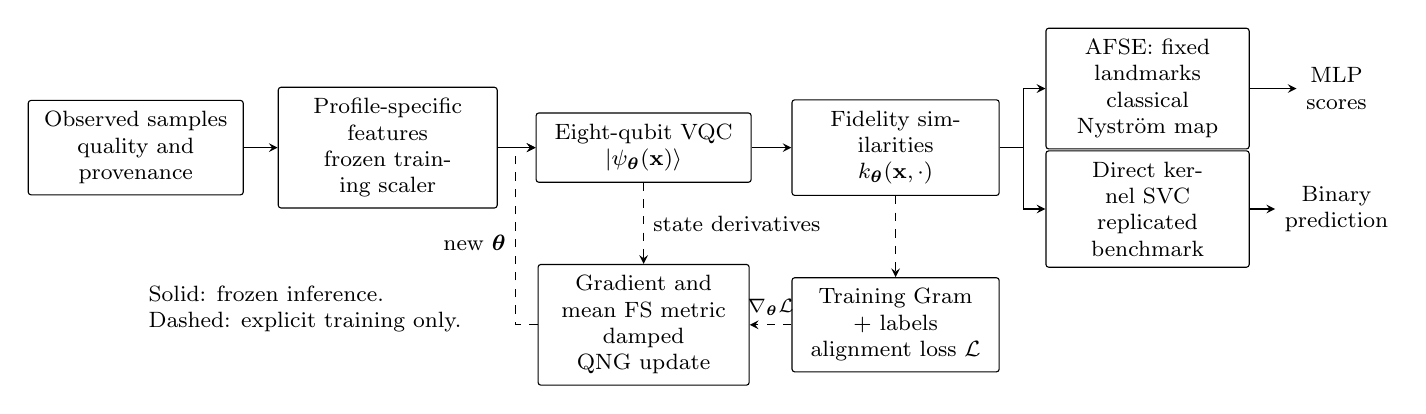
\begin{tikzpicture}[x=1cm,y=1cm,>=stealth,
  box/.style={draw,rounded corners=1pt,align=center,font=\footnotesize,inner sep=4pt,minimum height=0.82cm},
  small/.style={font=\footnotesize,align=center}]
\node[box,text width=2.45cm] (obs) at (0,0) {Observed samples\\quality and provenance};
\node[box,text width=2.50cm] (feat) at (3.20,0) {Profile-specific features\\frozen training scaler};
\node[box,text width=2.45cm] (state) at (6.45,0) {Eight-qubit VQC\\$\lvert\psi_{\boldsymbol\theta}(\mathbf x)\rangle$};
\node[box,text width=2.35cm] (kernel) at (9.65,0) {Fidelity similarities\\$k_{\boldsymbol\theta}(\mathbf x,\cdot)$};
\draw[->] (obs)--(feat); \draw[->] (feat)--(state); \draw[->] (state)--(kernel);
\node[box,text width=2.3cm] (afse) at (12.85,0.75) {AFSE: fixed landmarks\\classical Nystr\"om map};
\node[box,text width=2.3cm] (svm) at (12.85,-0.78) {Direct kernel SVC\\replicated benchmark};
\draw[->] (kernel.east) -- ++(0.30,0) |- (afse.west);
\draw[->] (kernel.east) -- ++(0.30,0) |- (svm.west);
\node[small] (mlp) at (15.25,0.75) {MLP\\scores};
\node[small] (binary) at (15.25,-0.78) {Binary\\prediction};
\draw[->] (afse.east)--(mlp.west); \draw[->] (svm.east)--(binary.west);
\node[box,text width=2.35cm] (loss) at (9.65,-2.25) {Training Gram + labels\\alignment loss $\mathcal L$};
\node[box,text width=2.4cm] (qng) at (6.45,-2.25) {Gradient and mean FS metric\\damped QNG update};
\draw[->,dashed] (kernel.south)--(loss.north);
\draw[->,dashed] (loss.west)-- node[above,font=\scriptsize] {$\nabla_{\boldsymbol\theta}\mathcal L$} (qng.east);
\draw[->,dashed] (state.south)-- node[right,font=\footnotesize] {state derivatives} (qng.north);
\draw[->,dashed] (qng.west)-- ++(-0.28,0) |- node[pos=0.23,left,font=\footnotesize] {new $\boldsymbol\theta$} (state.west);
\node[small,align=left] at (2.15,-2.05) {Solid: frozen inference.\\Dashed: explicit training only.};
\end{tikzpicture}
\caption{AQSE processing boundaries. The network demonstrator uses State8 and the AFSE--MLP branch. The 30-replica experiment uses harmonic features and the direct-kernel SVC branch. Labels enter the training objective, not the observed feature vector. The mean Fubini--Study (FS) metric is computed from state derivatives, separately from the loss gradient. No simulator truth enters inference.}
\label{fig:aqse-routes}
\end{figure*}


\subsection{Observations and Feature Profiles}
\label{sec:framework-observations}

A simulated network contains $N_s\in\{1,\ldots,8\}$ nodes. Each vector reading includes three measured field components, a timestamp, observed temperature, orientation, calibration identity, and quality flags. Simulator truth is retained separately. It may define experimental labels but is not an input to the feature extractor or predictor. The number of nodes is independent of the eight input coordinates and eight qubits. A circuit represents one accepted feature vector, not one qubit per sensor.

The demonstrator uses \emph{State8}, with separate local and network profiles. Let $R_i[k]$ map world-frame vectors to the sensor frame. The observed world-North component is
\begin{equation}
 b_i[k]=\mathbf e_N^{\mathsf T}R_i[k]^{\mathsf T}
             \mathbf B_i^{\mathrm{obs}}[k],
 \label{eq:north-observation}
\end{equation}
converted to nanotesla before feature extraction. This rotation uses the declared orientation. It does not infer or correct an unknown calibration error. At 100~Hz, an initial 800-sample reference freezes the mean North field $\bar b_{i,0}$ and temperature $\bar T_{i,0}$. Subsequent 400-sample windows advance by 100 samples. Within a window, define $d_i[k]=b_i[k]-\bar b_{i,0}$, with $k=0,\ldots,399$. Table~\ref{tab:state8} specifies the coordinates. Each accepted window uses only measurements acquired by its endpoint.

\begin{table}[t]
\caption{State8 coordinates in the network demonstrator. The local and network profiles share $x_0$--$x_4$ and $x_7$.}
\label{tab:state8}
\centering
\footnotesize
\setlength{\tabcolsep}{3pt}
\renewcommand{\arraystretch}{1.15}
\begin{tabular}{@{}cll@{}}
\toprule
Index & Definition & Unit\\
\midrule
$x_0$ & $\operatorname{mean}_k d_i[k]$ & nT\\
$x_1$ & $1.4826\operatorname{median}_k|d_i[k]-\operatorname{median}d_i|$ & nT\\
$x_2$ & Least-squares slope of $d_i[k]$ versus time & nT/s\\
$x_3$ & $10\log_{10}(\max(P_L,\epsilon)/\max(P_H,\epsilon))$ & dB\\
$x_4$ & $\operatorname{mean}_k T_i[k]-\bar T_{i,0}$ & K\\
\midrule
\multicolumn{3}{@{}l}{Local profile}\\
$x_5$ & $\sqrt{\operatorname{mean}_k(d_i[k+1]-d_i[k])^2}$ & nT\\
$x_6$ & $\operatorname{corr}(d_i[0{:}399],d_i[1{:}400])$ & 1\\
\midrule
\multicolumn{3}{@{}l}{Network profile}\\
$x_5$ & $\sqrt{\operatorname{mean}_k(d_i[k]-\operatorname{median}_{j\in\mathcal P_i}d_j[k])^2}$ & nT\\
$x_6$ & $|\mathcal P_i|^{-1}\sum_{j\in\mathcal P_i}\operatorname{corr}(d_i,d_j)$ & 1\\
\midrule
$x_7$ & Received vector samples / 400 & 1\\
\bottomrule
\end{tabular}
\par\smallskip
\begin{minipage}{\columnwidth}\footnotesize
$P_L$ and $P_H$ integrate a linearly detrended, Hann-windowed one-sided periodogram over $[0.25,2)$ and $[2,20]$~Hz. The power floor is $\epsilon=10^{-12}$~nT$^2$. Correlations are Pearson coefficients. Slice endpoints are exclusive.
\end{minipage}
\end{table}


For the network profile, the peer set $\mathcal P_i$ contains at least two other nodes with complete, aligned windows and valid references. With fewer valid peers, the runtime uses the compatible local path or abstains. One or two nodes do not support the network attribution task. Missing, stuck, clipped, or temporally inconsistent readings are not replaced by valid zeros. Undefined correlations also prevent the corresponding profile from entering inference. Under the implemented complete-window eligibility policy, the received fraction $x_7$ equals one for accepted windows; it remains informative in the quality record of rejected windows. An initial reference defines a measured baseline, not a certified normal state.

The replicated benchmark uses a different, harmonic feature vector,
\begin{equation}
 \mathbf x^{\mathrm{harm}}=
 (A,\phi,f,v,d,\mathrm{SNR},P_{\mathrm{peak}},T)^{\mathsf T},
 \label{eq:harmonic-vector}
\end{equation}
whose entries are oscillation amplitude, phase, frequency, variance, drift, signal-to-noise ratio, peak power spectral density (nT$^2$/Hz), and temperature. These are the extractor's fixed coordinates, not State8 coordinates. Each simulated episode contributes one predetermined window. The experiment therefore tests noise-regime classification through a direct kernel SVC. It does not measure the network demonstrator's causal attribution or AFSE classifier performance.

\subsection{Training-Only Scaling and Angle Encoding}
\label{sec:framework-encoding}

For each coordinate $j$, the shared \texttt{AngleScaler} stores the training mean $\mu_j$ and population standard deviation $\sigma_j$. It sets $s_j=\sigma_j$ when $\sigma_j>10^{-12}$ and $s_j=1$ otherwise. Its bounded map is
\begin{equation}
 a_j(\mathbf x)=\frac{\pi}{2}
    \tanh\!\left(\frac{x_j-\mu_j}{2s_j}\right),
 \qquad j=0,\ldots,7.
 \label{eq:angle-scaler}
\end{equation}
State8 uses~\eqref{eq:angle-scaler} on all eight coordinates. The harmonic benchmark instead replaces its phase coordinate by
\begin{equation}
 a_1(\mathbf x^{\mathrm{harm}})
   =\operatorname{wrap}_{[-\pi,\pi)}(\phi)
   =((\phi+\pi)\bmod 2\pi)-\pi.
 \label{eq:phase-direct}
\end{equation}
The other seven outputs remain unchanged. This convention respects phase periodicity but does not establish a common clock or cross-sensor phase reference. The harmonic phase is relative to the start of its window. Scaler parameters are fitted once on the relevant training population and remain fixed for validation, test, and subsequent queries. Neither query batching nor landmark selection refits them. The two encoding policies define different input spaces and are not interchangeable.

\subsection{Variational Circuit and Fidelity Kernel}
\label{sec:framework-kernel}

The circuit starts in $\lvert0\rangle^{\otimes8}$. Write its 16 parameters as $\boldsymbol\theta=(\boldsymbol\alpha,\boldsymbol\beta)$, where $\alpha_q=\theta_q$ and $\beta_q=\theta_{8+q}$. Define
\begin{equation}
 D_\nu(\mathbf a)=\bigotimes_{q=0}^{7}R_\nu(a_q),
 \qquad
 V_\nu(\boldsymbol\gamma)=\bigotimes_{q=0}^{7}R_\nu(\gamma_q),
 \label{eq:circuit-layers}
\end{equation}
for $\nu\in\{y,z\}$. With operators acting from right to left,
\begin{align}
 U_{\boldsymbol\theta}(\mathbf a)
  &=D_z(\mathbf a)V_y(\boldsymbol\beta)E
                  V_z(\boldsymbol\alpha)D_y(\mathbf a),
 \label{eq:vqc-unitary}\\
 \lvert\psi_{\boldsymbol\theta}(\mathbf x)\rangle
  &=U_{\boldsymbol\theta}(\mathbf a(\mathbf x))
                         \lvert0\rangle^{\otimes8}.
 \label{eq:encoded-state}
\end{align}
The entangler $E$ applies the even CZ edges $(0,1)$, $(2,3)$, $(4,5)$, and $(6,7)$ first, followed by $(1,2)$, $(3,4)$, and $(5,6)$. The graph is a path, not a ring. Figure~\ref{fig:tqk8-circuit} gives the gate sequence. A state preparation contains 32 single-qubit rotations and seven CZ gates. Every input angle appears twice; every trainable parameter appears once.

\begin{figure*}[t]
\centering
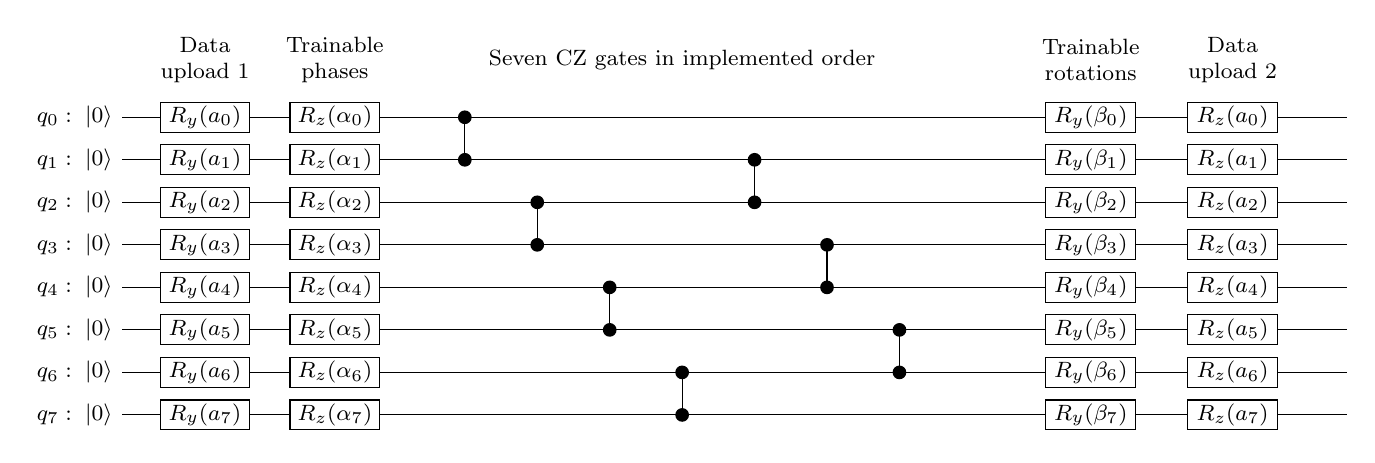
\begin{tikzpicture}[x=1cm,y=0.54cm,gate/.style={draw,fill=white,minimum width=1.14cm,minimum height=0.38cm,inner sep=1pt,font=\footnotesize},dot/.style={circle,fill,inner sep=1.75pt}]
\draw (0,0) -- (15.55,0);
\node[left,font=\footnotesize] at (0,0) {$q_0:\;\lvert0\rangle$};
\node[gate] at (1.05,0) {$R_y(a_0)$};
\node[gate] at (2.7,0) {$R_z(\alpha_0)$};
\node[gate] at (12.30,0) {$R_y(\beta_0)$};
\node[gate] at (14.10,0) {$R_z(a_0)$};
\draw (0,-1) -- (15.55,-1);
\node[left,font=\footnotesize] at (0,-1) {$q_1:\;\lvert0\rangle$};
\node[gate] at (1.05,-1) {$R_y(a_1)$};
\node[gate] at (2.7,-1) {$R_z(\alpha_1)$};
\node[gate] at (12.30,-1) {$R_y(\beta_1)$};
\node[gate] at (14.10,-1) {$R_z(a_1)$};
\draw (0,-2) -- (15.55,-2);
\node[left,font=\footnotesize] at (0,-2) {$q_2:\;\lvert0\rangle$};
\node[gate] at (1.05,-2) {$R_y(a_2)$};
\node[gate] at (2.7,-2) {$R_z(\alpha_2)$};
\node[gate] at (12.30,-2) {$R_y(\beta_2)$};
\node[gate] at (14.10,-2) {$R_z(a_2)$};
\draw (0,-3) -- (15.55,-3);
\node[left,font=\footnotesize] at (0,-3) {$q_3:\;\lvert0\rangle$};
\node[gate] at (1.05,-3) {$R_y(a_3)$};
\node[gate] at (2.7,-3) {$R_z(\alpha_3)$};
\node[gate] at (12.30,-3) {$R_y(\beta_3)$};
\node[gate] at (14.10,-3) {$R_z(a_3)$};
\draw (0,-4) -- (15.55,-4);
\node[left,font=\footnotesize] at (0,-4) {$q_4:\;\lvert0\rangle$};
\node[gate] at (1.05,-4) {$R_y(a_4)$};
\node[gate] at (2.7,-4) {$R_z(\alpha_4)$};
\node[gate] at (12.30,-4) {$R_y(\beta_4)$};
\node[gate] at (14.10,-4) {$R_z(a_4)$};
\draw (0,-5) -- (15.55,-5);
\node[left,font=\footnotesize] at (0,-5) {$q_5:\;\lvert0\rangle$};
\node[gate] at (1.05,-5) {$R_y(a_5)$};
\node[gate] at (2.7,-5) {$R_z(\alpha_5)$};
\node[gate] at (12.30,-5) {$R_y(\beta_5)$};
\node[gate] at (14.10,-5) {$R_z(a_5)$};
\draw (0,-6) -- (15.55,-6);
\node[left,font=\footnotesize] at (0,-6) {$q_6:\;\lvert0\rangle$};
\node[gate] at (1.05,-6) {$R_y(a_6)$};
\node[gate] at (2.7,-6) {$R_z(\alpha_6)$};
\node[gate] at (12.30,-6) {$R_y(\beta_6)$};
\node[gate] at (14.10,-6) {$R_z(a_6)$};
\draw (0,-7) -- (15.55,-7);
\node[left,font=\footnotesize] at (0,-7) {$q_7:\;\lvert0\rangle$};
\node[gate] at (1.05,-7) {$R_y(a_7)$};
\node[gate] at (2.7,-7) {$R_z(\alpha_7)$};
\node[gate] at (12.30,-7) {$R_y(\beta_7)$};
\node[gate] at (14.10,-7) {$R_z(a_7)$};
\draw (4.35,0) -- (4.35,-1);
\node[dot] at (4.35,0) {};
\node[dot] at (4.35,-1) {};
\draw (5.27,-2) -- (5.27,-3);
\node[dot] at (5.27,-2) {};
\node[dot] at (5.27,-3) {};
\draw (6.19,-4) -- (6.19,-5);
\node[dot] at (6.19,-4) {};
\node[dot] at (6.19,-5) {};
\draw (7.11,-6) -- (7.11,-7);
\node[dot] at (7.11,-6) {};
\node[dot] at (7.11,-7) {};
\draw (8.03,-1) -- (8.03,-2);
\node[dot] at (8.03,-1) {};
\node[dot] at (8.03,-2) {};
\draw (8.95,-3) -- (8.95,-4);
\node[dot] at (8.95,-3) {};
\node[dot] at (8.95,-4) {};
\draw (9.87,-5) -- (9.87,-6);
\node[dot] at (9.87,-5) {};
\node[dot] at (9.87,-6) {};
\node[font=\footnotesize,align=center] at (1.05,1.35) {Data\\upload 1};
\node[font=\footnotesize,align=center] at (2.7,1.35) {Trainable\\phases};
\node[font=\footnotesize] at (7.11,1.35) {Seven CZ gates in implemented order};
\node[font=\footnotesize,align=center] at (12.30,1.35) {Trainable\\rotations};
\node[font=\footnotesize,align=center] at (14.10,1.35) {Data\\upload 2};
\end{tikzpicture}
\caption{Protected TQK8 state-preparation circuit, read from left to right. Here $a_q$ is an encoded feature, $\alpha_q=\theta_q$, and $\beta_q=\theta_{8+q}$. A line with two filled endpoints denotes CZ. The seven gates are drawn sequentially to preserve the source order; no hardware schedule or transpiled depth is implied. The circuit has no measurement in exact-state evaluation.}
\label{fig:tqk8-circuit}
\end{figure*}


The shared-parameter fidelity kernel in~\eqref{eq:fidelity-kernel} can also be written as
\begin{equation}
 k_{\boldsymbol\theta}(\mathbf x,\mathbf x')=
 \operatorname{Tr}\!\left[\rho_{\boldsymbol\theta}(\mathbf x)
                           \rho_{\boldsymbol\theta}(\mathbf x')\right],
 \label{eq:density-kernel}
\end{equation}
where $\rho_{\boldsymbol\theta}(\mathbf x)=\lvert\psi_{\boldsymbol\theta}(\mathbf x)\rangle\langle\psi_{\boldsymbol\theta}(\mathbf x)\rvert$. This Hilbert--Schmidt inner product establishes positive semidefiniteness~\cite{schuld2019feature,havlicek2019supervised}. Exact normalized states give $k(\mathbf x,\mathbf x)=1$ and $0\leq k\leq1$. The final data-dependent layer in~\eqref{eq:vqc-unitary} prevents the circuit from reducing to a feature map followed solely by a common trainable unitary. Such a terminal unitary would cancel from the overlap and could not train the kernel.

The implementation provides independent NumPy and Qiskit statevector engines. The replicated study uses NumPy exact-state evaluation, without shots, hardware noise, or QPU submission. An ancilla-free overlap circuit is also defined: prepare $U_{\boldsymbol\theta}(\mathbf a)$, apply $U_{\boldsymbol\theta}(\mathbf a')^\dagger$, and measure the all-zero probability. Its existence is not evidence of a hardware experiment. The direct binary kernel classifier has decision function
\begin{equation}
 f(\mathbf x)=\sum_{i\in\mathcal S}c_i y_i
                k_{\boldsymbol\theta}(\mathbf x_i,\mathbf x)+b,
 \label{eq:kernel-svc}
\end{equation}
where $\mathcal S$ indexes the fitted support vectors. In the replicated benchmark, circuit optimization uses 32 balanced training examples, whereas the SVC uses all 72 training examples.

\subsection{Alignment Objective and Quantum Natural Gradient}
\label{sec:framework-qng}

For a binary training bank of size $M$, let $K_{\boldsymbol\theta}$ be its Gram matrix, $\mathbf y\in\{-1,+1\}^{M}$ its target vector, and $H=I_M-\mathbf1\mathbf1^{\mathsf T}/M$. The implemented objective is one minus centered kernel--target alignment~\cite{cortes2012alignment,hubregtsen2022training}:
\begin{align}
 K_c&=HK_{\boldsymbol\theta}H,
 &Y_c&=(H\mathbf y)(H\mathbf y)^{\mathsf T},\nonumber\\
 \mathcal L(\boldsymbol\theta)
   &=1-\frac{\langle K_c,Y_c\rangle_F}
                 {\|K_c\|_F\,\|Y_c\|_F}.
 \label{eq:alignment-loss}
\end{align}
The implementation rejects a centered kernel or target norm below $10^{-12}$. Labels enter this objective, not the observation vector. The loss is a training surrogate. It is not the SVC objective or a held-out accuracy measure.

Because each parameter occurs once in a Pauli rotation, the state derivative used by the exact simulator is
\begin{equation}
 \partial_r\lvert\psi_{\boldsymbol\theta}(\mathbf x)\rangle
 =\frac{
 \lvert\psi_{\boldsymbol\theta+\frac{\pi}{2}\mathbf e_r}(\mathbf x)\rangle
 -\lvert\psi_{\boldsymbol\theta-\frac{\pi}{2}\mathbf e_r}(\mathbf x)\rangle}
 {2\sqrt{2}}.
 \label{eq:state-derivative}
\end{equation}
This is an amplitude derivative, not the usual probability-shift formula. If $o_{ij}=\langle\psi_i\mid\psi_j\rangle$, then
\begin{equation}
 \partial_r K_{ij}=2\operatorname{Re}\!\left[
 o_{ij}^{*}\big(\langle\partial_r\psi_i\mid\psi_j\rangle
          +\langle\psi_i\mid\partial_r\psi_j\rangle\big)\right].
 \label{eq:kernel-derivative}
\end{equation}
Both occurrences of the shared parameter contribute to the gradient.

AQSE uses the empirical mean Fubini--Study metric~\cite{stokes2020qng}:
\begin{equation}
 \bar g_{rs}=\frac{1}{M}\sum_{i=1}^{M}\operatorname{Re}\!\left[
 \langle\partial_r\psi_i\mid\partial_s\psi_i\rangle
 -\langle\partial_r\psi_i\mid\psi_i\rangle
  \langle\psi_i\mid\partial_s\psi_i\rangle\right].
 \label{eq:mean-fs}
\end{equation}
No factor of four is applied. The implementation forms the full $16\times16$ matrix, then symmetrizes it numerically. This is a chosen state-space preconditioner. It is not asserted to be the unique natural metric of the kernel matrix or classifier.

Let $\mathbf h=\nabla_{\boldsymbol\theta}\mathcal L$. A tentative step is
\begin{align}
 \mathbf v&=\eta(\bar g+\lambda_g I_{16})^{-1}\mathbf h,\nonumber\\
 \boldsymbol\delta&=\min\!\left(1,\frac{\delta_{\max}}{\|\mathbf v\|_2}\right)
                 \mathbf v,
 \label{eq:damped-qng}
\end{align}
with $\eta=0.2$, $\lambda_g=10^{-3}$, and $\delta_{\max}=0.4$. A candidate $\boldsymbol\theta-\boldsymbol\delta$ is accepted only if
\begin{equation}
 \mathcal L(\boldsymbol\theta-\boldsymbol\delta)
 \leq\mathcal L(\boldsymbol\theta)-10^{-4}
                       \mathbf h^{\mathsf T}\boldsymbol\delta.
 \label{eq:armijo-qng}
\end{equation}
The step is halved after rejection, with at most 12 candidate evaluations per update. A gradient norm below $10^{-10}$ or failure to accept a step stops optimization. The study permits at most ten accepted updates and preserves the initial checkpoint. Optimizer coordinates are not wrapped or clamped after an update.

The target is task-specific. The harmonic study uses nominal versus elevated noise labels. The demonstrator's local loss uses normal versus change labels. Its network loss uses only environment-compatible versus device-compatible training examples. Normal and mixed examples are excluded from that binary optimization bank but remain available to the downstream four-class model. Thus, network QNG does not directly optimize the four-class prediction loss.

\subsection{Fixed-Landmark AFSE Representation}
\label{sec:framework-afse}

The demonstrator converts kernel similarities into a fixed-dimensional vector using a regularized Nystr\"om map~\cite{williams2001nystrom}. AQSE calls this interface AFSE. It is a classical transformation of quantum-kernel evaluations, not a second quantum circuit.

Let $\mathcal Z=(\mathbf z_1,\ldots,\mathbf z_m)$ be an ordered, class-balanced set of training landmarks, with one distinct generative lineage per landmark. The requested size is 32. If training support is insufficient, the implementation reduces $m$ while retaining class balance; the output dimension then equals the recorded $m\leq32$. Landmark identities, order, encoding, and $\boldsymbol\theta$ are frozen together. Define
\begin{align}
 W_{ij}&=k_{\boldsymbol\theta}(\mathbf z_i,\mathbf z_j),
 &\mathbf k_{\mathcal Z}(\mathbf x)_j
    &=k_{\boldsymbol\theta}(\mathbf x,\mathbf z_j),\nonumber\\
 W&=Q\operatorname{diag}(\boldsymbol\lambda)Q^{\mathsf T}.
 \label{eq:landmark-gram}
\end{align}
An eigenvalue below $-10^{-10}\max(1,\lambda_{\max})$ causes rejection. Smaller numerical negatives are clipped to zero, giving $\lambda_j^+=\max(\lambda_j,0)$. The stored symmetric inverse square root is
\begin{equation}
 B=Q\operatorname{diag}\!\left((\lambda_j^++\lambda_N)^{-1/2}\right)
       Q^{\mathsf T},\qquad \lambda_N=10^{-6}.
 \label{eq:nystrom-basis}
\end{equation}
The column-vector embedding and its induced approximate kernel are
\begin{align}
 \mathbf z(\mathbf x)&=B\mathbf k_{\mathcal Z}(\mathbf x),
 \label{eq:afse-map}\\
 \widetilde k(\mathbf x,\mathbf x')
   &=\mathbf k_{\mathcal Z}(\mathbf x)^{\mathsf T}B^2
                              \mathbf k_{\mathcal Z}(\mathbf x').
 \label{eq:afse-kernel}
\end{align}
For row-oriented batches, the implementation evaluates $K_{X\mathcal Z}B$. A query's coordinates depend on the frozen representation, not on other queries in the batch. The regularization and finite landmark set mean that $\widetilde k$ need not equal $k_{\boldsymbol\theta}$.

The diagnostic residual is
\begin{equation}
 r(\mathbf x)=k_{\boldsymbol\theta}(\mathbf x,\mathbf x)
                    -\|\mathbf z(\mathbf x)\|_2^2.
 \label{eq:afse-residual}
\end{equation}
Values below $-10^{-10}$ are rejected; smaller numerical negatives are set to zero. The runtime flags a query when its residual exceeds the empirical training 99th percentile. This is a reference-coverage heuristic. It is neither a calibrated out-of-distribution test nor evidence of a physical fault. Training landmarks are included in the population used to set that threshold. AFSE is absent from the replicated direct-kernel benchmark.

\subsection{Classical Output and Runtime Boundaries}
\label{sec:framework-runtime}

The demonstrator standardizes AFSE vectors using training statistics and fits a multilayer perceptron with hidden widths 32 and 16. With standardized input $\widehat{\mathbf z}$, its logits are
\begin{equation}
 \mathbf u=W_3\tanh\!\left(W_2\tanh(W_1\widehat{\mathbf z}+\mathbf b_1)
                  +\mathbf b_2\right)+\mathbf b_3.
 \label{eq:mlp-logits}
\end{equation}
Binary output uses a sigmoid; four-class output uses a softmax. Fitting uses L-BFGS and an $L_2$ regularization coefficient of $10^{-3}$. A raw-State8 baseline uses the same hidden widths with separately fitted training preprocessing. It has a different input dimension and is not parameter-count matched to the AFSE model. This baseline is also distinct from the 11-parameter MLP in the replicated experiment.

The local task reports normal or change. The network task reports normal, environment-compatible, device-compatible, or mixed/ambiguous patterns. These labels express similarity to simulated training conditions, not identified physical causes. A top score below 0.70 or a top-two score margin below 0.15 produces an uncertainty status. Quality failures and incompatible representations can instead cause abstention. Scores are not treated as calibrated probabilities.

A model bundle binds the feature profile, fitted scaler, encoding policy, exact circuit parameters, landmarks, AFSE basis, downstream standardizer, and classifier. Applying a different bundle invalidates cached representations and pending results from the previous one. Training is explicit and cancellable between optimizer calls. It does not run at every measurement or backend restart. Simulation time, data transport, and analysis cadence are separate. The inference worker uses a bounded buffer and a newest-window queue, reporting result age, skipped windows, and latency. These controls make the computation auditable; they do not establish real-time guarantees or field diagnostic accuracy.

\section{Experimental Methodology}
\label{sec:methodology}

\subsection{Scope and Prespecified Protocol}
\label{sec:methods-scope}

The 30-replica study evaluates the harmonic-feature TQK--SVC route, not the network State8--AFSE--MLP route. Its task is discrimination of nominal and elevated white-noise regimes. Each replica comprises a new simulated corpus, an episode-level split, optimization, model selection, and held-out evaluation. Dataset, split, QNG, and classical-model randomness vary together; their separate variance contributions are not identified~\cite{aqse2026canonical}.

The protocol was recorded in the source repository on September 16, 2026, before the primary execution. We use \emph{preregistered} to denote this repository-level record, not an external registration service. It fixes the replica counts, seed rules, model budgets, and primary decision criterion. There is no performance-based stopping or extension of the primary study. An earlier four-run negative-control pilot informed the choice of 12 subsequent control runs. That pilot is excluded from the reported groups. The control count was thus informed by prior observations. No prospective power calculation is specified.

The primary criterion requires a positive lower endpoint of the 95\% interval for the mean paired TQK-minus-RBF TEST balanced-accuracy difference and two-sided Wilcoxon $p<0.05$. Macro-F1 and the other comparators are secondary and cannot replace this criterion. No equivalence margin or hardware-speed criterion is defined.

\subsection{Simulated Episodes and Harmonic Features}
\label{sec:methods-data}

Each primary replica contains 120 independent episode lineages, with 60 episodes per noise regime. Every episode uses a static vector magnetometer at the origin, an identity linear response, and a constant background field of $(20{,}000,0,45{,}000)$~nT. A sinusoidal perturbation is applied along the $x$ axis. The generator samples amplitude, frequency, initial phase, temperature, and noise standard deviation from the distributions in Table~\ref{tab:benchmark-domain}. The nuisance distributions are the same for both labels. Nominal noise defines $y=-1$ and elevated noise defines $y=+1$. The configured standard deviation is applied to each measured component as Gaussian white noise per sample. It is not a noise spectral density. The configuration has no injected bias, deterministic drift, random walk, Ornstein--Uhlenbeck component, dropout, thermal bias, or bandwidth filter.

\begin{table}[t]
\caption{Primary magnetometer corpus. All uniform draws are made per episode; nuisance ranges are shared by both labels.}
\label{tab:benchmark-domain}
\centering
\footnotesize
\setlength{\tabcolsep}{3pt}
\begin{tabular}{@{}p{0.43\columnwidth}p{0.52\columnwidth}@{}}
\toprule
Quantity & Fixed value or distribution \\
\midrule
Primary replicas & 30 new corpora \\
Episodes per corpus & 120 (60 per class) \\
TRAIN / VALIDATION / TEST & 72 / 24 / 24 episodes \\
Episode acquisition & 10 s, 100 Hz, 1,000 samples \\
Harmonic amplitude & $A\sim\mathcal U(6,10)$ nT \\
Harmonic frequency & $f\sim\mathcal U(4,8)$ Hz \\
Initial phase & $\phi\sim\mathcal U(-\pi,\pi)$ rad \\
Constant temperature & $T\sim\mathcal U(292.15,294.15)$ K \\
Nominal noise ($y=-1$) & $\sigma_\epsilon\sim\mathcal U(0.25,0.75)$ nT (per sample) \\
Elevated noise ($y=+1$) & $\sigma_\epsilon\sim\mathcal U(1.5,3.0)$ nT (per sample) \\
Component clipping limit & $800~\mu$T in absolute value \\
Feature window / hop & 1 s / 0.5 s \\
Retained window & Ordinal 9, samples $[450,550)$ \\
QNG bank / SVC fit & 32 balanced rows / all 72 TRAIN rows \\
\bottomrule
\end{tabular}
\end{table}


Each episode contains 1,000 samples at 100~Hz, at times $0,0.01,\ldots,9.99$~s. The extractor uses only the observed $x$ component, converted from tesla to nanotesla, and observed temperature. It forms complete 100-sample windows with a 50-sample hop. Of the 19 resulting windows, only zero-based ordinal 9 is retained for learning. This is the index interval $[450,550)$, or $[4.5,5.5)$~s. Thus each episode contributes one eight-dimensional row. Overlapping windows are not counted as independent examples. The injected parameters define the simulation and label but are not substituted for feature estimates.

The harmonic extractor in~\eqref{eq:harmonic-vector} first removes a least-squares intercept and linear trend for spectral estimation. It computes a Hann-windowed, one-sided power spectral density and estimates the dominant non-DC frequency by bounded parabolic peak interpolation. A regression of the original window onto an intercept, centered time, sine, and cosine at that estimated frequency supplies amplitude, phase, and drift. Phase is relative to the window start. SNR is the ratio of fitted periodic power to residual power, expressed in decibels with numerical floors and clipping to $[-300,300]$~dB. Variance is the population variance of the observed signal. Peak PSD excludes the DC bin, and temperature is averaged within the window.

Eligibility requires a nonconstant signal, at least two estimated cycles, peak prominence of at least 6~dB over the median non-DC PSD, harmonic SNR of at least 0~dB, and no clipped samples. Nonuniform or nonfinite input is rejected. If the predetermined window is missing or ineligible, the replica raises an error. It does not substitute another window, regenerate an episode until it passes, or silently omit the row. This task measures classification within the specified harmonic/noise domain, not general fault diagnosis.

\subsection{Splits, Seeds, and Information Boundaries}
\label{sec:methods-splits}

Episode lineages are assigned before simulation to a stratified 60/20/20 split. Each class contributes 36 TRAIN, 12 VALIDATION, and 12 TEST episodes, giving partition sizes of 72, 24, and 24. Lineage and episode identifiers cannot cross partitions. Rows are ordered by episode identifier after assignment. The same rows and labels are supplied to all five methods within a replica; no cross-validation folds are used.

The primary base seed is 3001001. For replica $r$ and domain $d$, the implementation hashes the UTF-8 string \texttt{aqse-paper-v1:b:r:d}, substituting the decimal base seed $b$ and replica index $r$. The first four SHA-256 bytes, interpreted as an unsigned little-endian integer, define the seed. Domains distinguish replica identity, dataset generation, splitting, QNG, classical fitting, and permutation control. Within episode generation, separate hash namespaces drive nuisance parameters, the noise intervention, and measurement noise. All derived seeds are recorded. Domain separation defines reproducible pseudorandom streams.

Scaler fitting uses TRAIN only. VALIDATION selects configurations but is never appended to TRAIN for refitting. The selected predictor is then applied to TEST without further fitting. The run stores a selection record before the designated TEST loader is invoked. Its ledger has the ordered events \texttt{sealed}, \texttt{observations\_opened}, \texttt{labels\_opened}, and \texttt{evaluation\_published}. Predictions are computed after loading test features and before the designated label load. The last event binds the published result by SHA-256.

This is a workflow guard rather than an inaccessible holdout service: test arrays exist in the dataset container, and structural validation checks their shapes and class support. Fitting uses only the training and validation fields. The ledger records the designated loader sequence, not every possible memory access. It guards against accidental reuse within this implementation and is not a security proof.

\subsection{Quantum Model Selection and Classical Comparators}
\label{sec:methods-models}

The TQK uses the circuit, centered-alignment objective, and damped QNG update of Section~\ref{sec:framework}. The scaler is fitted to all 72 training rows. The harmonic phase override in~\eqref{eq:phase-direct} is then applied. A seeded, without-replacement sample of 16 training rows per class forms the fixed 32-row QNG bank. All 16 initial circuit parameters are drawn uniformly from $[-0.8,0.8]$ using the replica QNG seed.

At most ten QNG updates are accepted, with learning rate 0.2, damping $10^{-3}$, and maximum step norm 0.4. The line search and termination tests remain those of the protected implementation. Checkpoint 0 is the initial circuit. Each accepted update contributes another checkpoint; no update is inserted when the optimizer stops. For each checkpoint, the SVC is fitted on the full, uncentered $72\times72$ TRAIN fidelity Gram matrix for $C\in\{0.1,1,10\}$. Centering is used in the alignment objective, not in the SVC input. Selection maximizes validation balanced accuracy, then macro-F1. Exact ties favor the earlier checkpoint and then smaller $C$. The maximum search budget is 33 checkpoint--$C$ candidates per replica. Only the selected checkpoint is evaluated on TEST. This study does not include a separately selected fixed-kernel or ordinary-gradient TEST arm.

\begin{table*}[t]
\caption{Frozen model configurations. The TQK and RBF use VALIDATION for selection. Other comparator configurations are fixed. All predictors are fitted on the same full TRAIN partition; the 32-row restriction applies only to QNG.}
\label{tab:comparator-budget}
\centering
\footnotesize
\setlength{\tabcolsep}{4pt}
\begin{tabular}{@{}p{0.12\textwidth}p{0.24\textwidth}p{0.40\textwidth}p{0.16\textwidth}@{}}
\toprule
Method & Input and preprocessing & Fitting configuration & Candidate budget \\
\midrule
TQK--SVC & Eight-angle map; TRAIN-fitted scaler; direct periodic phase & 8 qubits, 16 parameters; at most 10 QNG updates; uncentered fidelity kernel; $C\in\{0.1,1,10\}$ & Up to $11\times3=33$ \\
RBF-SVC & Eight raw features; TRAIN standardization & $C\in\{0.1,1,10\}$; $\gamma\in\{0.01,0.1,1\}$ & $3\times3=9$ \\
MLP-11 & Eight raw features; TRAIN standardization & One tanh hidden unit; L-BFGS; L2 coefficient $10^{-3}$; maximum 500 iterations & 1 \\
RFF-256 & Eight raw features; TRAIN standardization; 256 RBF random features & RFF $\gamma=0.125$; linear SVC $C=1$; maximum 10,000 iterations & 1 \\
Gradient boosting & Eight raw features, no standardization & 100 estimators; learning rate 0.1; maximum tree depth 3 & 1 \\
\bottomrule
\end{tabular}
\end{table*}


Table~\ref{tab:comparator-budget} specifies the four classical comparators. RBF-SVC, MLP, and RFF use a TRAIN-fitted standardizer on the original eight feature coordinates; gradient boosting uses those coordinates without standardization. In particular, the classical phase input remains a scalar in radians. These comparators do not use the nine-coordinate sine/cosine phase map of an earlier AQSE experiment. Shared observations therefore do not imply identical preprocessing.

RBF selection maximizes validation balanced accuracy and then macro-F1, with smaller $C$ and then smaller $\gamma$ breaking ties. The other three classical configurations are fixed; their validation scores are recorded but do not select a grid point. Library defaults not overridden in Table~\ref{tab:comparator-budget} are those of the recorded scikit-learn version. Search budgets are not equalized across families.

The one-hidden-unit binary MLP has 11 trainable weights and biases. This is a capacity reference, not a match to the full TQK--SVC predictor, which also learns support-vector coefficients and an intercept. Likewise, 256 RFF components match $2^8$ numerically, not the hypothesis class or computational cost of a fidelity kernel. No parameter-count, runtime, or representational equivalence is assumed.

\subsection{Mechanism-Aligned and Training-Label Controls}
\label{sec:methods-controls}

Both controls use synthetic eight-dimensional examples, not magnetometer episodes. They retain the same model-fitting and selection procedures, but their stratified partition sizes are 120/40/40, with equal class counts. Their outputs are reported separately from the primary study.

\subsubsection{Mechanism-aligned positive control}
The positive-control base seed is 3003001. Each of its 12 runs constructs a new 200-example dataset using the replica dataset seed. Candidate coordinates are sampled uniformly from $[-1.4,1.4]^8$. A teacher circuit uses the protected VQC with parameters drawn from $[-0.8,0.8]^{16}$ using \texttt{SeedSequence([dataset\_seed,17])}. For two fixed prototype vectors $\mathbf p_-$ and $\mathbf p_+$, define
\begin{equation}
 h(\mathbf x)=k_{\boldsymbol\theta^{\rm teach}}(\mathbf x,\mathbf p_+)
              -k_{\boldsymbol\theta^{\rm teach}}(\mathbf x,\mathbf p_-).
 \label{eq:teacher-control}
\end{equation}
The label is $+1$ for $h(\mathbf x)\geq0$ and $-1$ otherwise. Candidates are drawn in batches of 200 until at least 100 exist in each class. The 100 largest absolute contrasts per class are retained, then shuffled and split. The released generator specifies the prototype coordinates. This selection creates a class-balanced, margin-enriched control rather than an unfiltered uniform sample. Teacher labels precede the student's TRAIN-fitted encoding; exact teacher realizability by the student is not assumed.

\subsubsection{TRAIN-label permutation control}
One teacher-generated dataset of 200 examples is constructed with seed 3004001. All 12 negative-control runs reuse this dataset. Base seed 3002001 supplies new splits, QNG and classical seeds, and TRAIN-label permutations. The per-run dataset seed does not generate a fresh corpus. Sample identities may recur across runs but not across partitions within a run.

Only TRAIN labels are permuted. Correct VALIDATION labels still select the TQK checkpoint and $C$, and the RBF hyperparameters. TEST labels remain unchanged. The protocol's diagnostic criterion is whether each method's 95\% mean balanced-accuracy interval contains 0.5. It is not a formal equivalence test or a full label-null experiment. Its resampling variability is conditional on the one control dataset, not variability over 12 independently generated corpora. This distinction is retained when interpreting the control.

\subsection{Metrics and Statistical Analysis}
\label{sec:methods-statistics}

For each replica and method, the recorded metrics are balanced accuracy and macro-F1. With class-wise counts $\mathrm{TP}_c$, $\mathrm{FP}_c$, and $\mathrm{FN}_c$, they are
\begin{align}
 \mathrm{BA}&=\frac{1}{2}\sum_{c\in\{-1,+1\}}
 \frac{\mathrm{TP}_c}{\mathrm{TP}_c+\mathrm{FN}_c},\label{eq:balanced-accuracy}\\
 F_{1,\mathrm{macro}}&=\frac{1}{2}\sum_{c\in\{-1,+1\}}
 \frac{2\mathrm{TP}_c}{2\mathrm{TP}_c+\mathrm{FP}_c+\mathrm{FN}_c}.
 \label{eq:macro-f1}
\end{align}
Undefined class-wise F1 terms are assigned zero. Both true classes are required in every partition. In the balanced 24-episode primary TEST, a single additional correct prediction changes BA by $1/24$; this discreteness produces ties and limits per-replica resolution.

The primary inferential unit is the replica, not a window or a method--replica row. For baseline $m$, the paired effect is
\begin{equation}
 \Delta_{r,m}=\mathrm{BA}_{r,\mathrm{TQK}}-\mathrm{BA}_{r,m},
 \qquad \bar\Delta_m=\frac{1}{30}\sum_{r=0}^{29}\Delta_{r,m}.
 \label{eq:paired-effect}
\end{equation}
An analogous difference is calculated for macro-F1. The report includes mean, median, sample standard deviation, minimum, and maximum for method scores and paired differences. It also records the fraction of strictly positive paired differences.

The percentile bootstrap resamples replica-level values with replacement 2,000 times~\cite{efron1979bootstrap}. Paired intervals resample the within-replica differences, not the two methods independently. The 2.5th and 97.5th percentiles of the resampled means use linear interpolation. Inputs are sorted before resampling; endpoints are expanded to include the observed mean if needed. Intervals are neither bias-corrected nor studentized. Primary mean-score seeds are $3011001+10j+q$; paired-difference seeds are $3021001+10j+q$. Here $q=0$ for BA and $q=1$ for macro-F1. Method order is TQK, RBF, MLP, RFF, and boosting; paired order omits TQK. The group aggregates and kernel summaries have separately recorded hash-derived bootstrap seeds.

The paired Wilcoxon signed-rank test is two-sided, with Pratt zero handling and the recorded SciPy \texttt{method="auto"} implementation~\cite{wilcoxon1945ranking,pratt1959zeros}. Exactly zero differences enter ranking and their signed contributions are omitted. If all differences are exactly zero, the wrapper returns $p=1$. The test is computed from unrounded floating-point scores, without tolerance-based merging of near-ties. Reproduction of the frozen test therefore requires that numerical convention. The signed-rank null concerns the distribution of paired differences about zero; it is not itself a test of the mean in~\eqref{eq:paired-effect}.

The prespecified criterion combines the paired mean interval and the Wilcoxon result. Secondary comparisons and intervals are reported without a built-in family-wise adjustment. Any multiplicity correction, spectral--performance correlation, or checkpoint-stratified analysis added during manuscript analysis must be identified as post hoc. None changes the frozen primary criterion or model selection.

\subsection{Kernel Diagnostics and Computational Records}
\label{sec:methods-diagnostics}

Every available checkpoint supplies an uncentered TRAIN Gram matrix for spectral analysis. Let $\lambda_i^+=\max(\lambda_i,0)$, $\tau=\sum_i\lambda_i^+$, and $p_i=\lambda_i^+/\tau$. The recorded summaries include
\begin{equation}
 r_{\rm eff}=\exp\!\left(-\sum_{i:p_i>0}p_i\log p_i\right),
 \qquad c_{\rm spec}=\frac{\max_i\lambda_i^+}{\tau}.
 \label{eq:kernel-spectrum-diagnostics}
\end{equation}
The entropy-based effective rank follows~\cite{roy2007rank}. Symmetry errors above $10^{-10}$ are rejected. The matrix is symmetrized for eigendecomposition, and eigenvalues below $-10^{-9}\max(1,\max_i|\lambda_i|)$ cause rejection. Only residual negative roundoff is clipped for the entropy calculation. The reported positive-spectrum condition number excludes eigenvalues no larger than $10^{-12}\max(1,\max_i|\lambda_i|)$; it is not an unconditional condition number for a rank-deficient matrix.

The archive retains the full spectrum, diagonal and off-diagonal summaries, and the selected checkpoint identity. TEST--TRAIN cross-kernels have shape $24\times72$ in the primary study and $40\times120$ in the controls; their minimum, maximum, mean, and standard deviation are recorded after selection. Kernel geometry describes the representation, not a separate accuracy criterion. No TEST metric for an unselected checkpoint is generated. The records therefore do not provide a trained-versus-initial TEST ablation.

Timers separate dataset generation, joint training/model selection, and joint test evaluation. The total runtime is repeated in each method row of \texttt{replicas.csv}; it is not a per-method runtime. These records do not support a method-specific speed comparison.

\subsection{Execution Provenance and Report Recovery}
\label{sec:methods-provenance}

The experiment ran offline in the backend container using NumPy exact-state simulation, without GUI interaction, finite-shot sampling, or QPU access. The recorded environment is Python 3.12.14, NumPy 2.5.3, SciPy 1.18.1, scikit-learn 1.9.0, and Qiskit 2.5.2 on Linux/aarch64. Qiskit was installed but was not the backend used for the replicated computation. The scientific execution revision is \texttt{091acf2}; the published code-and-results snapshot is \texttt{0ed58cf}~\cite{aqse2026canonical}.

A JSON serialization failure occurred after replica evaluation. A separate report-only recovery at revision \texttt{d42965e} read the persisted results and completed aggregation and packaging. It did not regenerate data, refit models, make new predictions, or reload TEST arrays. Source evidence was hashed before and after recovery. The canonical \texttt{report-recovery-v2} package includes full commit identifiers, protocol, environment, per-replica records, diagnostics, and manifest. The earlier noncanonical report package is excluded. Experimental and reporting provenance remain distinct.

\section{Results}
\label{sec:results}

\subsection{Completed Evaluation and Primary Comparison}
\label{sec:results-primary}

The released record contains all 30 primary replicas, 12 TRAIN-label control runs, and 12 positive-control runs, with no recorded replica failures. These groups are not pooled. The primary results concern the harmonic-feature TQK--SVC benchmark described in Section~\ref{sec:methods-scope}, not the network State8--AFSE--MLP demonstrator. All statistics in Tables~\ref{tab:main-performance} and~\ref{tab:paired-results} retain the canonical reporting conventions. The new descriptive and association analyses below use published scores and diagnostics, without new model fits or TEST predictions~\cite{aqse2026canonical}.

% Generated from canonical aggregate_statistics.json. Do not hand-edit numbers.
\begin{table*}[t]
\caption{Held-out performance across 30 primary replicas. Brackets are the canonical 95\% percentile-bootstrap intervals for the mean; SD is the sample standard deviation across replicas.}
\label{tab:main-performance}
\centering
\small
\setlength{\tabcolsep}{5pt}
\begin{tabular}{lcccccc}
\toprule
& \multicolumn{3}{c}{Balanced accuracy} & \multicolumn{3}{c}{Macro-F1} \\
\cmidrule(lr){2-4}\cmidrule(lr){5-7}
Method & Mean & 95\% interval & SD & Mean & 95\% interval & SD \\
\midrule
TQK & 0.9528 & [0.9333, 0.9708] & 0.0544 & 0.9523 & [0.9312, 0.9707] & 0.0556 \\
RBF-SVC & 0.9569 & [0.9444, 0.9694] & 0.0371 & 0.9568 & [0.9428, 0.9694] & 0.0373 \\
MLP-11 & 0.9750 & [0.9639, 0.9861] & 0.0321 & 0.9749 & [0.9624, 0.9861] & 0.0322 \\
RFF-256 & 0.9472 & [0.9292, 0.9653] & 0.0512 & 0.9468 & [0.9282, 0.9651] & 0.0519 \\
Gradient boosting & 0.9806 & [0.9708, 0.9903] & 0.0284 & 0.9805 & [0.9707, 0.9902] & 0.0285 \\
\bottomrule
\end{tabular}
\end{table*}

% Canonical unadjusted inference; W/T/L is a descriptive post hoc count.
\begin{table*}[t]
\caption{Paired TEST comparisons. Differences are TQK minus baseline. Intervals and unadjusted two-sided Pratt--Wilcoxon $p$-values are canonical. W/T/L denotes balanced-accuracy wins, ties, and losses with tolerance $10^{-12}$; this tolerance is not used to recompute the canonical tests.}
\label{tab:paired-results}
\centering
\small
\setlength{\tabcolsep}{4.5pt}
\begin{tabular}{lccccl}
\toprule
Baseline & Metric & Mean difference & 95\% interval & $p$ & BA W/T/L \\
\midrule
RBF-SVC (primary) & BA & -0.0042 & [-0.0222, +0.0125] & 0.9328 & 10/10/10 \\
 & Macro-F1 & -0.0045 & [-0.0226, +0.0125] & 0.9162 &  \\
\addlinespace[2pt]
MLP-11 & BA & -0.0222 & [-0.0444, -0.0014] & 0.0311 & 4/13/13 \\
 & Macro-F1 & -0.0226 & [-0.0442, -0.0027] & 0.0731 &  \\
\addlinespace[2pt]
RFF-256 & BA & +0.0056 & [-0.0194, +0.0306] & 0.5560 & 11/10/9 \\
 & Macro-F1 & +0.0055 & [-0.0183, +0.0311] & 0.5014 &  \\
\addlinespace[2pt]
Gradient boosting & BA & -0.0278 & [-0.0486, -0.0083] & 0.0166 & 5/11/14 \\
 & Macro-F1 & -0.0282 & [-0.0497, -0.0083] & 0.0431 &  \\
\bottomrule
\end{tabular}
\end{table*}


The mean TEST balanced accuracy was 0.9528 for TQK and 0.9569 for the primary RBF-SVC baseline. The paired mean difference was $-0.0042$, or $-0.42$ percentage points, with a 95\% bootstrap interval of $[-0.0222,0.0125]$. The two-sided Pratt--Wilcoxon statistic was 201.0, with $p=0.9328$. Neither condition of the preregistered predictive-advantage criterion was met. This result does not establish equivalence: no equivalence margin was specified, and the interval includes both positive and negative differences.

TQK exceeded RBF in ten replicas, tied it in ten, and fell below it in ten. These descriptive counts treat absolute score differences no larger than $10^{-12}$ as ties. The canonical bootstrap and Wilcoxon calculations retain the original unrounded values. This distinction matters for one TQK--MLP pair that differs only at floating-point roundoff; it does not alter the primary comparison.

\begin{figure}[t]
\centering
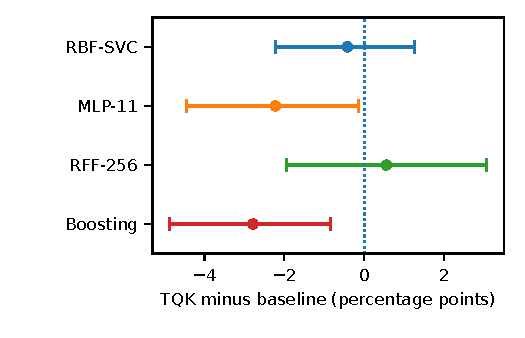
\includegraphics[width=\columnwidth]{figures/results_paired_delta.pdf}
\caption{Primary-study paired balanced-accuracy differences, expressed in percentage points. Points and bars are the canonical mean differences and 95\% bootstrap intervals. Only the RBF-SVC balanced-accuracy comparison defines the preregistered primary criterion. The other comparisons are secondary.}
\label{fig:results-paired}
\end{figure}

\subsection{Secondary Metrics and Between-Replica Variation}
\label{sec:results-variation}

The largest mean balanced accuracy was 0.9806 for gradient boosting, followed by 0.9750 for MLP-11, 0.9569 for RBF-SVC, 0.9528 for TQK, and 0.9472 for RFF-256. Macro-F1 had the same ordering. For TQK versus RBF, the macro-F1 difference was $-0.0045$ with interval $[-0.0226,0.0125]$ and $p=0.9162$.

The secondary TQK-minus-MLP and TQK-minus-boosting balanced-accuracy differences were $-0.0222$ and $-0.0278$, with unadjusted $p=0.0311$ and $p=0.0166$, respectively. TQK minus RFF was $0.0056$, with interval $[-0.0194,0.0306]$ and $p=0.5560$. The two negative secondary intervals are not simultaneous confidence intervals. For macro-F1, the corresponding TQK--MLP and TQK--boosting unadjusted $p$-values were 0.0731 and 0.0431.

As a post-hoc multiplicity sensitivity check, applying Holm's procedure~\cite{holm1979multiple} to all four balanced-accuracy comparisons gives adjusted $p=0.0664$ for boosting and $p=0.0932$ for MLP. Restricting that family to the three secondary comparisons instead gives 0.0498 and 0.0621. Neither family definition was preregistered. We retain the raw secondary results and disclose this dependence on the testing family rather than using a retrospective family choice to make a confirmatory claim.

\begin{figure}[t]
\centering
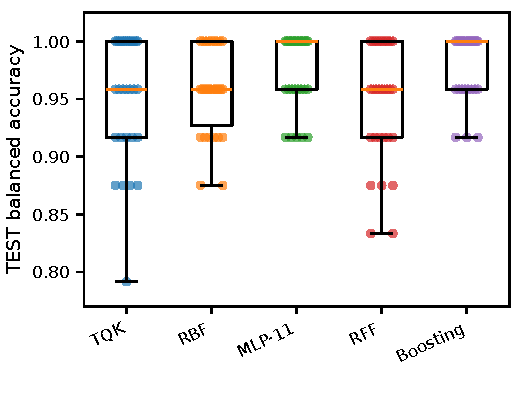
\includegraphics[width=\columnwidth]{figures/results_performance.pdf}
\caption{TEST balanced accuracy in all 30 primary replicas per method. Boxes show medians and interquartile ranges; whiskers extend to observations within 1.5 interquartile ranges. Every observation is plotted, including those outside the whiskers. Horizontal spreading separates tied scores and does not change their values.}
\label{fig:results-performance}
\end{figure}

TQK had the largest observed between-replica standard deviation, 0.0544, compared with 0.0371 for RBF and 0.0284 for boosting. It reached balanced accuracy 1 in 13 of 30 replicas but fell below 0.90 in five. The corresponding below-0.90 counts were two for RBF, zero for MLP, five for RFF, and zero for boosting. The minimum TQK score was 0.7917 in replica 15. This replica is retained in every reported aggregate. Figure~\ref{fig:results-performance} shows the score distributions; no test of equal variances is used. These descriptive differences cannot isolate dataset, split, or initialization effects because those sources of randomness vary together.

\subsection{Kernel Geometry and Checkpoint Selection}
\label{sec:results-kernel}

The primary archive contains 330 TRAIN-kernel diagnostic records: the initial checkpoint and ten accepted updates in each of 30 replicas. VALIDATION selected checkpoint 0 in 19 replicas and an updated checkpoint in 11. The nonzero selections were checkpoint 1 once, checkpoint 2 four times, checkpoint 3 once, checkpoint 4 twice, checkpoint 5 once, and checkpoint 7 twice. No selected checkpoint was chosen from TEST performance.

Across the selected $72\times72$ uncentered Gram matrices, the mean effective rank was 28.8241, with a 95\% interval of $[28.0758,29.5220]$. The mean largest-eigenvalue share, $c_{\rm spec}$, was 0.2160, with interval $[0.2076,0.2243]$, and the trace was approximately 72. Selected effective ranks ranged from 24.9784 to 32.7250; selected spectral concentrations ranged from 0.1746 to 0.2676. These finite-sample summaries differ from both a rank-one limit and an identity Gram matrix. They do not measure circuit expressivity or establish predictive generalization.

\begin{figure}[t]
\centering
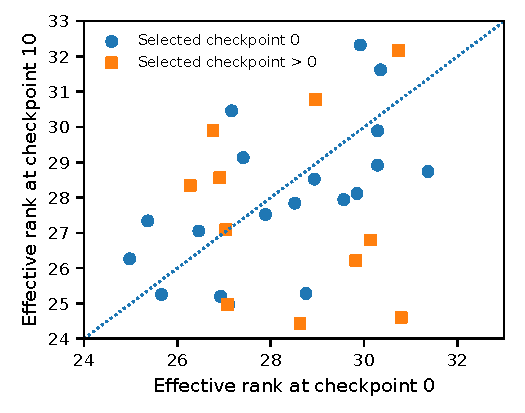
\includegraphics[width=\columnwidth]{figures/results_rank_change.pdf}
\caption{Initial versus checkpoint-10 effective rank for all 30 primary replicas. The dotted line denotes equal rank. Marker shape indicates whether VALIDATION selected the initial or an updated checkpoint; the vertical coordinate always refers to checkpoint 10. This is a comparison of stored kernel diagnostics, not a trained-versus-untrained TEST comparison.}
\label{fig:results-rank-change}
\end{figure}

Comparing checkpoint 10 with checkpoint 0, effective rank increased in 13 replicas and decreased in 17. Its mean change was $-0.4566$, while the mean absolute change was 1.9701; individual changes ranged from $-6.1879$ to $3.2980$. Spectral concentration increased in nine replicas and decreased in 21, with mean change $-0.0096$. Thus optimization changed the recorded spectral summaries without a common direction of effective-rank change (Fig.~\ref{fig:results-rank-change}). The archive does not contain TEST evaluations of the unselected initial models. It therefore cannot estimate the paired predictive effect of QNG relative to a fixed initial kernel. Selecting an updated checkpoint is not a substitute for that comparison.

\subsection{Exploratory Geometry--Performance Associations}
\label{sec:results-correlations}

We examined four post-hoc associations: selected effective rank and spectral concentration against TQK TEST balanced accuracy and against its paired difference from RBF. Each analysis uses one selected diagnostic pair per replica, rather than treating the 330 checkpoints as independent observations. Spearman correlations use average ranks~\cite{spearman1904association}. For this analysis only, balanced accuracies are mapped to their verified integer counts on the $1/24$ grid, avoiding artificial rank distinctions due to floating-point roundoff.

% Exploratory analysis; not part of the preregistered criterion.
\begin{table}[t]
\caption{Post-hoc associations between selected-kernel geometry and TEST performance ($n=30$). $\rho_s$ is Spearman correlation; $p_{\rm MC}$ uses 19,999 random pairings with the add-one correction. All four Holm-adjusted values are 1.}
\label{tab:geometry-associations}
\centering
\small
\setlength{\tabcolsep}{4pt}
\begin{tabular}{llrr}
\toprule
Predictor & Endpoint & $\rho_s$ & $p_{\rm MC}$ \\
\midrule
$r_{\rm eff}$ & TQK BA & +0.154 & 0.410 \\
$r_{\rm eff}$ & $\Delta_{\rm TQK-RBF}$ & +0.069 & 0.712 \\
$c_{\rm spec}$ & TQK BA & -0.140 & 0.451 \\
$c_{\rm spec}$ & $\Delta_{\rm TQK-RBF}$ & -0.093 & 0.625 \\
\bottomrule
\end{tabular}
\end{table}


Two-sided association $p$-values use 19,999 random pairings and the add-one correction~\cite{phipson2010permutation}. The four permutation seeds are 4001001--4001004 in table order. Percentile intervals use 2,000 paired replica resamples with seeds 4002001--4002004. The input extracts, calculations, and interval endpoints are included with the manuscript sources. These procedures were defined during manuscript analysis and do not replace any frozen comparison.

The estimated correlations ranged from $-0.140$ to $0.154$, and the unadjusted permutation $p$-values ranged from 0.410 to 0.712 (Table~\ref{tab:geometry-associations}). All four Holm-adjusted $p$-values were 1.000. The intervals were broad. For example, effective rank versus TQK balanced accuracy had $\rho_s=0.154$ and interval $[-0.215,0.501]$. The observed selected-kernel summaries therefore do not resolve a monotonic association with performance in these 30 replicas. This does not exclude weaker, nonlinear, or task-dependent relationships.

\subsection{Control Results}
\label{sec:results-controls}

Table~\ref{tab:control-results} reports the two controls separately. Under TRAIN-label permutation, mean balanced accuracy was 0.6146 for TQK and 0.6271 for RBF. Their canonical intervals excluded 0.5. The intervals for MLP, RFF, and boosting included 0.5. The prespecified chance-compatibility check was therefore not met for the two validation-selected kernel methods. Inclusion of 0.5 for the other methods is not evidence of equivalence to chance.

% Exact control-summary extract, no new control evaluation.
\begin{table}[t]
\caption{Control balanced accuracy. Each cell gives the canonical mean and 95\% bootstrap interval. The negative-control intervals condition on one shared dataset.}
\label{tab:control-results}
\centering
\footnotesize
\setlength{\tabcolsep}{3pt}
\renewcommand{\arraystretch}{1.15}
\begin{tabular}{lcc}
\toprule
Method & TRAIN-label control & Positive control \\
\midrule
TQK & \shortstack{0.6146\\{}[0.5333, 0.6958]} & \shortstack{0.9813\\{}[0.9625, 0.9958]} \\
RBF-SVC & \shortstack{0.6271\\{}[0.5479, 0.7083]} & \shortstack{0.9792\\{}[0.9646, 0.9917]} \\
MLP-11 & \shortstack{0.5521\\{}[0.4750, 0.6292]} & \shortstack{0.9708\\{}[0.9542, 0.9875]} \\
RFF-256 & \shortstack{0.5104\\{}[0.4417, 0.5792]} & \shortstack{0.9688\\{}[0.9479, 0.9854]} \\
Grad. boosting & \shortstack{0.5354\\{}[0.4792, 0.5855]} & \shortstack{0.9333\\{}[0.9000, 0.9625]} \\
\bottomrule
\end{tabular}
\end{table}


These negative-control intervals describe randomized re-splits and permutations conditional on one teacher dataset. Correct VALIDATION labels remained available for checkpoint and hyperparameter selection. The result is thus a limitation of this TRAIN-label ablation, not an observation from a fully label-null pipeline. The present records do not establish why the two methods remained above chance, or establish TEST leakage.

In the positive control, TQK reached mean balanced accuracy 0.9813 and RBF reached 0.9792. Their paired difference was 0.0021, with interval $[-0.0083,0.0125]$ and $p=1.0000$. Against boosting, the difference was 0.0479, with interval $[0.0208,0.0771]$ and unadjusted $p=0.0117$. That control comparison is distinct from the primary sensor-task criterion. The data were generated by a TQK teacher and enriched for large fidelity contrasts. These results establish neither transfer to physical sensors nor a representation exclusive to the quantum method.

\subsection{Recorded Computation and Reproduction}
\label{sec:results-computation}

The recorded total runtimes of the 30 primary replicas sum to 312.94~s. The median was 10.38~s, with a range of 10.15--11.64~s. Each value includes dataset generation, fitting and selection across all methods, and their TEST evaluation. The repeated runtime field in the method-level CSV must be counted once per replica. It does not support a TQK-versus-classical timing comparison or a hardware-speed claim.

A report-only reconstruction of the ten method--metric summaries and eight paired summaries matched the canonical means, intervals, and signed-rank outputs to a maximum absolute difference of $2.8\times10^{-17}$. Tables retain the canonical values. The additional counts, endpoint geometry summaries, and association tests are identified as descriptive or post hoc. No simulations, quantum-state evaluations, training jobs, or TEST predictions were repeated for this section.

\section{Discussion}
\label{sec:discussion}

\subsection{Meaning of the Primary Result}
\label{sec:discussion-primary}

The primary study does not support a predictive advantage of the tested TQK over RBF-SVC. The paired estimate and its interval concern the complete fitting and selection procedures under the specified simulator distribution. They do not compare all possible quantum and classical models. The interval permits small effects in either direction, and no equivalence margin was specified. Neither the large Wilcoxon $p$-value nor the ten wins, ten ties, and ten losses establishes equality of the methods.

High absolute accuracy answers a different question. Both kernel methods classified the controlled noise regimes with mean balanced accuracy above 0.95, while MLP and gradient boosting had higher observed means. The task therefore supplies a discriminative signal that several classical model families can exploit. Its labels are determined by separated noise ranges, and its features include SNR, variance, and spectral power. This construction provides a controlled test of the representation, not evidence that classification requires quantum computation. The result belongs to the task-dependent empirical setting studied in quantum-kernel benchmarks~\cite{alvarez2025benchmarking,schnabel2025scrutiny}; it does not contradict learning separations established for different data constructions~\cite{liu2021rigorous}.

The secondary comparisons help describe this setting but do not replace the primary test. Their interpretation depends on the stated metric and testing family. Section~\ref{sec:results-variation} reports that dependence rather than choosing a post-hoc correction that supports a preferred conclusion. The observed ordering also cannot be attributed solely to parameter count: the TQK predictor includes a fitted SVC, and the search budgets and preprocessing differ across families.

\subsection{Geometric Change and Predictive Utility}
\label{sec:discussion-geometry}

The selected Gram matrices have spectral structure distinct from a rank-one matrix and from the identity matrix. This excludes those two simple descriptions of the recorded finite-sample kernels. It does not establish a general expressivity property, a favorable margin, or a generalization guarantee. Effective rank and largest-eigenvalue share depend on the kernel eigenvalues, not on the labels. Kernels with the same spectrum can have different alignments with a fixed label vector. Predictive utility consequently cannot be inferred from either scalar summary alone.

Three geometric objects must remain separate. The QNG preconditioner uses the empirical Fubini--Study metric of the parameterized states. The training objective uses centered kernel--target alignment. The reported spectra belong to uncentered TRAIN Gram matrices. The first preconditions a parameter update; improving the second is a training objective; changing the third is a descriptive observation. None is identical to improving held-out SVC accuracy~\cite{stokes2020qng,cortes2012alignment}.

The four exploratory correlations did not resolve a monotonic association between the selected spectral summaries and TEST performance. Their broad intervals do not establish that kernel geometry is irrelevant. They constrain what can be concluded from these two summaries in 30 realizations. The analysis used one selected kernel per replica and avoided treating correlated checkpoints as independent evidence. It also cannot establish an absence of concentration as qubit count grows. Concentration results concern specified embeddings, data distributions, and measurement resources~\cite{thanasilp2024concentration}; this experiment fixes eight qubits and evaluates exact statevectors.

\subsection{What Checkpoint Selection Reveals}
\label{sec:discussion-selection}

All trajectories contain ten accepted QNG updates, but VALIDATION retains the initial checkpoint in 19 replicas. This does not mean that 19 optimizations failed. The selection rule favors the earlier checkpoint when balanced accuracy and macro-F1 tie. An initial selection can therefore reflect a tie or a better validation score. Conversely, the 11 updated selections do not quantify a TEST improvement caused by training. The unselected initial predictors were not evaluated on TEST, so the required within-replica counterfactual scores are absent.

The objective and evaluation data also differ. Alignment is optimized on 32 training rows, whereas the SVC is fitted on all 72 training rows and selected using 24 validation episodes. The bank objective is not the SVC's held-out classification risk. Ten accepted steps establish execution of the prescribed optimizer, not convergence to an optimal embedding. Without a matched fixed-kernel or ordinary-gradient arm, the study cannot distinguish the effect of representation training from the effect of the QNG preconditioner.

The larger observed TQK dispersion motivates a robustness question, but does not answer its cause. Dataset generation, partition assignment, initialization, and model fitting vary together. Validation-based selection can itself be sensitive to finite samples~\cite{cawley2010selection}; the present data do not identify that mechanism as the source of the lower-scoring TQK replicas. We therefore retain all replicas and avoid interpreting the selection distribution as an optimizer ranking.

\subsection{Interpretation of the Controls}
\label{sec:discussion-controls}

The TRAIN-label control did not meet its prespecified chance-compatibility check for TQK and RBF. That finding remains a limitation, not a result to remove or relabel as a successful check. The implemented intervention breaks the training label assignment while preserving correct validation labels. TQK and RBF still use those labels to select among candidate models. Selection is part of the supervised procedure. A candidate fitted to permuted labels can be retained because its boundary happens to agree with validation structure. This is a plausible route to above-chance performance, not an explanation established by the recorded runs.

The fact that these two methods perform a configuration search is compatible with that hypothesis. It is not a controlled test of the hypothesis: the model families, preprocessing, and budgets differ, and no paired control removes validation supervision. The 12 runs also re-split one teacher-generated dataset. Their intervals describe randomization conditional on that dataset, not variation across newly sampled sensor corpora. The control therefore neither demonstrates TEST leakage nor certifies its absence. An audit claim about information isolation requires the recorded implementation and access sequence, not accuracy near chance alone.

The positive control addresses another boundary. It checks the fitting pipeline on examples whose labels derive from a TQK-teacher fidelity contrast. Retention of the largest contrasts enriches the margin, and the student applies its own fitted preprocessing. Success supports operation of the pipeline on this constructed signal. It does not establish a representation unavailable to classical kernels, as the primary RBF comparison within that control provides no supported TQK advantage. Neither control supplies evidence about physical magnetometer deployment.

\subsection{Implications for Contextual Sensor Processing}
\label{sec:discussion-framework}

AQSE provides an explicit interface between observations, feature profiles, a trainable kernel, and downstream models. Its engineering contribution is the separation and versioning of those interfaces, together with traceable evaluation. The quantum state represents an encoded classical feature vector. It is not a reconstruction of the sensor's microscopic state. Likewise, the AFSE coordinates are a classical Nystr\"om transformation of kernel similarities, not an additional quantum algorithm~\cite{williams2001nystrom}.

The replicated benchmark isolates the harmonic-feature TQK--SVC route. Its results cannot be assigned to the network State8--AFSE--MLP route, whose reference construction, features, embedding approximation, and classifier differ. A device moving through a spatial field may diverge from its peers without being faulty. Shared instrumental changes may resemble an environmental change. The framework therefore reports pattern compatibility and data-quality status rather than treating a class score as identification of a physical cause~\cite{aqse2026canonical}.

For the same reason, a high score or a small AFSE residual is not a deployment certificate. The residual threshold and score gates are engineering heuristics. Their false-alarm and abstention behavior must be evaluated on the complete acquisition and inference path. Versioned bundles make that path identifiable, but do not supply calibration or field validity. The practical implication of the current benchmark is to retain classical comparators for the same task output rather than assume that an added quantum representation improves the service.

\subsection{Follow-up Questions}
\label{sec:discussion-future}

A subsequent study could compare fixed initialization, ordinary-gradient training, and QNG on matched episodes and declared selection budgets. It should also compare circular phase preprocessing and simple noise-sensitive baselines, such as SNR or residual-variance rules. These would be new ablations, not retroactive replacements for the frozen study. A separate label-null control could permute TRAIN and VALIDATION labels before any model selection, using fresh datasets and a prospectively fixed analysis.

Extension to the application requires different evidence: complete network evaluation under motion and device perturbations, then measurements from physical sensors. Finite-shot or QPU evaluation would additionally require explicit accounting for state preparation, kernel estimation, optimization, and classical processing. These are proposed experiments. None was performed during manuscript analysis, and none changes the reported primary result.

\section{Limitations}
\label{sec:limitations}

\subsection{Domain and Sampling}

The primary data come from one controlled simulator configuration: a static magnetometer, harmonic excitation, two separated white-noise ranges, and one predetermined feature window per episode. Thirty new corpora measure repeatability within that generator. They do not sample different device technologies, sites, calibration states, or application tasks. The benchmark does not include motion, correlated disturbances, drift, missing data, or changing class prevalence. Its conclusions cannot be transferred to the network demonstrator or to field measurements without separate evaluation.

The finite samples limit precision. Each primary TEST contains 24 episodes and has balanced-accuracy resolution $1/24$. Some methods frequently attain the maximum score, reducing the range over which differences can be observed. No prospective power calculation or equivalence margin was specified. The percentile intervals quantify the recorded replication scheme, not uncertainty over all sensor environments or circuit designs.

\subsection{Model Comparison and Attribution}

The experiment fixes the circuit, encoding policy, ten-step optimization budget, QNG bank, and comparator configurations. TQK and RBF have different search spaces, while the other classical configurations are fixed. The quantum phase is treated periodically, whereas the classical phase remains a standardized scalar where standardization is used. Neither matched preprocessing nor matched computational budgets were tested. The 11 MLP parameters and 256 random features are reference counts, not equivalences to the full TQK--SVC hypothesis class. Strong performance on this task cannot establish a quantum contribution without the missing ablations.

Only the selected quantum model has TEST scores. The archive cannot support a paired estimate of training benefit, a QNG-versus-gradient comparison, or an attribution of performance differences to entanglement. It contains no scaling experiment in qubit count, depth, training size, or number of shots. Effective rank and spectral concentration describe finite Gram matrices, not asymptotic trainability or classical simulation hardness.

\subsection{Controls and Statistical Interpretation}

The negative control preserves validation supervision and reuses a single synthetic teacher dataset. It is not a full label-null control, and its failed chance check for two methods remains unresolved. The positive control is mechanism-aligned and margin-enriched. Both controls differ from the physical data-generating task and must remain separate from the primary evidence.

Secondary tests have no preregistered multiplicity correction. The sensitivity to retrospective family definitions is disclosed in Section~\ref{sec:results-variation}. Geometry--performance correlations are post hoc and imprecise; no discovered association was tested in a new dataset. The canonical Wilcoxon calculation also retains unrounded scores, so numerical near-ties can affect ranks. Its reproduction convention is preserved rather than silently changed. The bootstrap intervals are percentile intervals, not simultaneous, bias-corrected, or studentized bounds.

\subsection{Execution and Operational Evidence}

All quantum computations are exact statevector calculations on a classical backend. There is no finite-shot uncertainty, quantum-device noise, transpilation overhead, or QPU execution in the reported experiment. The recorded durations combine work across methods and cannot support a method-specific speed comparison. Sensor-noise simulation does not substitute for a quantum-hardware noise model.

The TEST ledger records a prescribed local workflow rather than enforcing an inaccessible holdout service. Test arrays exist in the process, and structural checks inspect their format and class support. Code review and provenance complement that guard; the ledger alone cannot prove absence of all unintended access. The report-only recovery preserves completed evaluations but adds no independent experimental evidence. Finally, the benchmark does not validate live alarm calibration, AFSE OOD detection, continuous adaptation, or hard real-time operation. These limits remain despite successful software execution.

\section{Conclusions}
\label{sec:conclusion}

AQSE connects versioned sensor-feature representations to an eight-qubit trainable fidelity kernel and classical prediction interfaces. A repository-preregistered experiment evaluated its harmonic-feature TQK--SVC component across 30 newly generated sensor corpora. The mean balanced accuracy was 0.9528 for TQK and 0.9569 for RBF-SVC. The paired difference was $-0.0042$ with a 95\% bootstrap interval of $[-0.0222,0.0125]$. The primary predictive-advantage criterion was not met.

QNG changed the recorded kernel spectra, but those changes do not establish a benefit in held-out prediction. Selected-kernel geometry was distinct from rank-one and identity limits, while the exploratory spectral--performance associations remained unresolved. The TRAIN-label control retained validation supervision and did not meet the chance-compatibility check for TQK and RBF. It therefore cannot serve as a complete label-null validation.

The contribution is a traceable framework and a bounded comparative evaluation, not evidence of quantum hardware advantage or field readiness. The study separates representational change from predictive benefit and preserves the negative and inconclusive findings. Future matched ablations and physical-sensor studies can test extensions without altering this frozen evidence.


\bibliographystyle{IEEEtran}
\bibliography{bibliography}
\end{document}
